\documentclass{beamer}
\usepackage{amsmath}
\usepackage{listings}
\usepackage{pgfplots}
\usepackage{xcolor}
\usetheme{Boadilla}
\author{Scott Cotton}
\title{Reach: Formal Verification in Go}

\institute{Independent}
\date{\today}
\begin{document}

\begin{frame}
\titlepage
\end{frame}

\section{Formal Verification in Go}

\subsection{Reach: Overview}
\begin{frame}
	\frametitle{Reach: What's the Problem?}
	\begin{center}
		\large{$$(x,I,T,B)$$}
	\includegraphics[width=0.8\textwidth]{fsis.png}

	\begin{itemize}
		\item Infinite traces.
		\item Symbolic, ergo big state space $2^{|x|}$.
		\item PSPACE complete.
		\item Fundamental and inescapable.
	\end{itemize}
	\end{center}

\end{frame}

\begin{frame}
	\frametitle{Core Approaches ($\sim$Orthogonal)}
	\begin{columns}
		\column{0.33\textwidth}
		\center{Sim}\\


		\begin{itemize}
			\item Main tool for exploration.
			\item Non-exhaustive.
			\item Finds most bugs that BMC finds.
			\item {\em Very} fast.
			\item Very well understood.
		\end{itemize}

		\column{0.33\textwidth}
		\center{BMC}\\
		\begin{itemize}
				\item Exhaustive for finite prefix.
				\item Long prefix $\implies$ high confidence.
				\item Can produce counterexamples.
				\item Understood.
				\item Often very fast.
		\end{itemize}

		\column{0.33\textwidth}
		\center{Proofs}\\
		\begin{itemize}
			\item Complete safety.
			\item Certificates.
			\item Not well understood.
			\item Many methods (IMC, TI, \ldots)
			\item Incremental induction!
		\end{itemize}

	\end{columns}
\end{frame}

\begin{frame}
	\frametitle{Reach: the tool}
	\begin{center}
	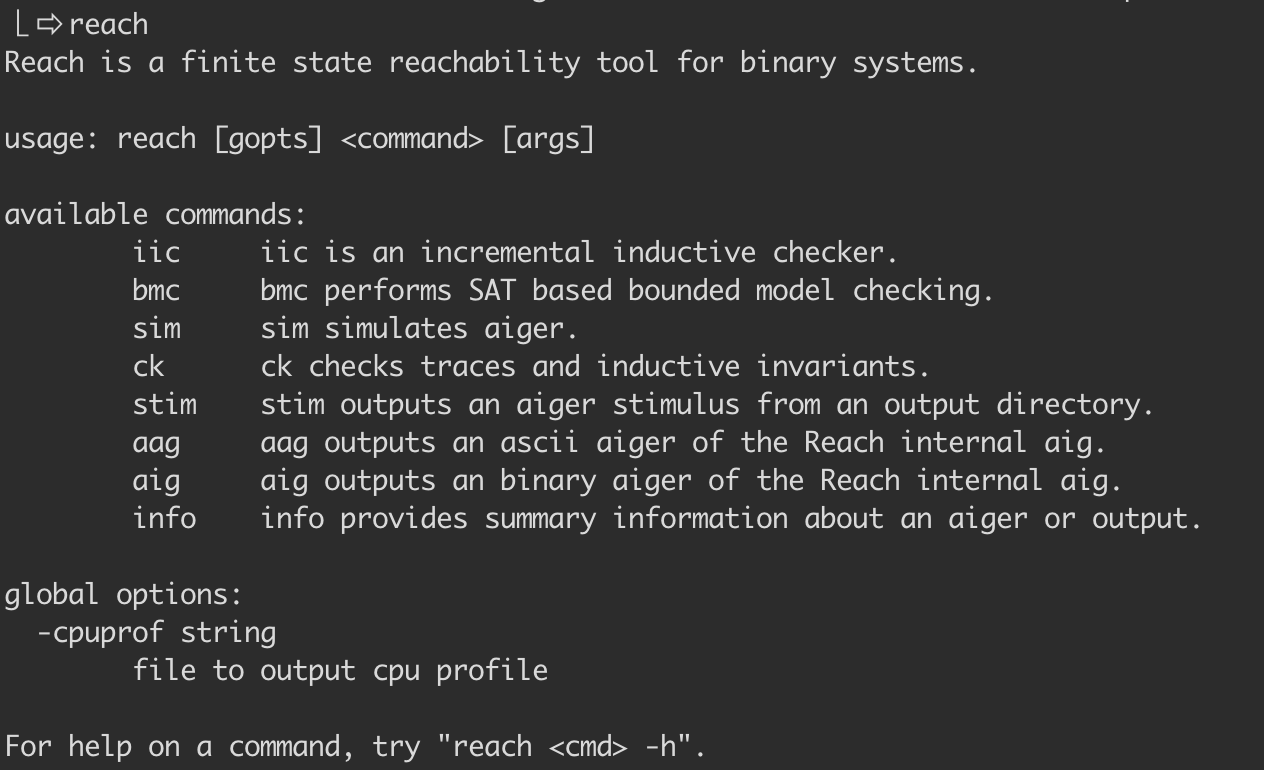
\includegraphics[width=0.8\textwidth]{reach.png}
	\end{center}
\end{frame}

\begin{frame}
	\frametitle{Focus: Proofs {\em via} SAT solving}
	\begin{itemize}
		\item Proofs are only true solution to the reachability problem.
		\item IIC: incremental inductive checking.
		\item Existential queries $\implies$ no space brick wall.
		\item Use Gini \url{http://www.github.com/irifrance/gini}.
		\item Exploit incremental scoping, activation literals.
	\end{itemize}
\end{frame}


\subsection{Focus on Proofs}
\begin{frame}
	\frametitle{Proofs: Incremental Induction}
	\begin{center}
		\em{Good ideas are contagious.}
	\end{center}
	\begin{itemize}
		\item Aaron Bradley (2007-present)
		\item Alan Mischenko, Niklas Een ABC PDR (2010-present)
		\item Nikolai Bjorner Z3 PDR with Horn clauses (?)
		\item $\ldots$
	\end{itemize}
\end{frame}

\begin{frame}
	\frametitle{Incremental Induction}
	\begin{columns}
		\column{0.5\textwidth}
		\begin{center}Induction\end{center}
		Find $P$:
		\begin{align*}
			I & \implies & P\\
			P & \implies & \neg B\\
			P \wedge T & \implies & P'
		\end{align*}
		How to find $P$?

		Temporal induction: use the post-image of a BMC prefix.\\
		Interpolation: use interpolant of a BMC prefix with $\neg B$.
		\column{0.5\textwidth}
		\begin{center}Incremental\end{center}
		Given $A$, find $P$:
		\begin{align*}
			I & \implies & P\\
			P & \implies & \neg b\\
			A \wedge P \wedge T & \implies & P'
		\end{align*}
		Then update $A \leftarrow A \wedge P$.

		In PDR/IC3, $A$ is CNF, $P$ is a clause which blocks
		states than can reach $B$, indicated above as $b$.
	\end{columns}
\end{frame}

\subsubsection{Incremental Induction Core Ideas}
\begin{frame}
	\frametitle{Incremental Induction -- CNFs}
To check reachability with incremental induction, we maintain a levelled CNF
	\[
		\Gamma \circeq \bigcup_i \Gamma_i, i \in [1\ldots K]
	\]
with
	\[
		\Gamma_i \equiv \bigwedge_j \bigvee M_j, M_j \subseteq \{ m | m \equiv v \mbox{ or } m \equiv \neg v, v \in x \}
	\]
\begin{itemize}
	\item Each $\Gamma_i$ represents an {\em overapproximation} of the reachable states
		from $\Gamma_{i-1}$ (or from $I$ for $\Gamma_1$).
	\item Syntactically, as a set of clauses, $\Gamma_i \supseteq \Gamma_{i+1}$
	\item Semantically, $\Gamma_i \subseteq \Gamma_{i+1}$
	\item Let $\lambda_i \circeq \Gamma_i \setminus (\bigcup_{j> i} \Gamma_j)$.
		These are clauses local to level $i$.
	\item Inversely, we can define $\Gamma_i$ in terms of $\lambda_i$:
		\[
			\Gamma_i \circeq \bigcup_{j \ge i} \lambda_j
			\]
\end{itemize}
\end{frame}

\begin{frame}[fragile]
	\frametitle{Incremental Induction -- Algorithm}
	\begin{itemize}
		\item IC3 and PDR are $2$-phase algorithms.
		\item Blocking phase: find inductive clauses incrementally from 
			bad state backward reachable states.
		\item Propagation phase: identify when clauses become relatively inductive.
	\end{itemize}
	\begin{lstlisting}[basicstyle=\small]
	// check I => not(B), I and T => not(B')
	initialize() 
	k := 1
	for {
		if not block(k)  {
			return Reachable
		}
		if propagate(k) {
			return Unreachable
		}
		k++
	}
	\end{lstlisting}
\end{frame}

\begin{frame}
	\frametitle{Incremental Induction: Blocking}
	\begin{center}
		\includegraphics[height=0.5\textheight]{iic-block.png}
		\[ \begin{array}{|lcl|c|}
			\hline
			\mbox{CNF} &           & \mbox{clause} & \mbox{enabling condition}\\
			\hline
			\lambda_1 & \leftarrow & \top & \\
			\lambda_1 & \leftarrow & \lambda_1 \wedge \neg \alpha_1 & \mbox{sat}(\alpha_1 \wedge T \wedge B'), \mbox{unsat}(I \wedge T \wedge \alpha'_1) \\
			\lambda_2 & \leftarrow & \top & \mbox{unsat}(\Gamma_1 \wedge T \wedge B') \\
			\lambda_2 & \leftarrow & \lambda_2 \wedge \neg \alpha_2 & \mbox{sat}(\alpha_2 \wedge T \wedge (B' \vee \alpha'_1)),\mbox{unsat}(\Gamma_1 \wedge T \wedge \alpha'_2)\\
			\hline
		\end{array} \]
	\end{center}
\end{frame}

\begin{frame}
	\frametitle{Blocking: Lifting and Generalization}
	How do we find $\alpha_i$?
	\begin{enumerate}
		\item Maintain a tree of proof obligations.
		\item Each proof obligation is a term $o \equiv \bigwedge \{ a_0, a_1, \ldots \}$.
		\item Find $\sigma$ s.t. $\sigma$ can reach a bad state $b$
			from some $\Gamma_j$ (SAT problems).
		\item {\em Lift} $\sigma$ to a small term $o$ such every extension of $o$ can transition
			to $b$, independent of $\Gamma_j$. 
		\item Generalize $o$ by finding a small subclause which makes the query
			$$\Gamma_j \wedge \neg o \wedge T \wedge o'$$
			unsat.
	\end{enumerate}
		$\alpha_i$ is then the result of generalization.
\end{frame}

\begin{frame}
	\frametitle{Incremental Induction: Propagation}
Given $K$ levels $[1\ldots K]$, and a set of clauses $\Gamma_k$ for each
level $k$ such that

	\begin{center}
		\begin{align*}
			\Gamma_k & \implies \Gamma_{k+1}, &k \in [1\ldots K)\\
			I & \implies \Gamma_k, &k \in [1\ldots K]\\
			\Gamma_k \wedge T & \implies \Gamma_{k+1}, &k \in [1\ldots K)
		\end{align*}
	\end{center}

	Find the closure of the following consecution rule (CR) ($k \in [1 \ldots K]$)

	\begin{center}
		\begin{align*}
			\mbox{if }&c \in \Gamma_k, \Gamma_k \wedge T  \implies c'\\
			\mbox{then }&c \in \Gamma_{k+1}
		\end{align*}
	\end{center}

\end{frame}

\begin{frame}
	\frametitle{Incremental Induction: Termination}
	Suppose we propagate with $\Gamma_i, i \in [1\ldots K]$, and
	the result is that $\Gamma_K = \Gamma_{k+1}$.

	Then $\Gamma_K$ is an inductive invariant proving unreachability.

	\begin{align*}
		I \implies \Gamma_K\\
		\Gamma_K \implies \neg B\\
		\Gamma_K \wedge T \implies \Gamma'_K
	\end{align*}
\end{frame}


\begin{frame}
	\frametitle{Incremental Induction: The Reach Way}
	\begin{itemize}
			\item Justifying Proof Obligations.
			\item Sifting Generalization.
			\item Unified Queueing.
				\begin{itemize}
					\item Consecutive Sifting
					\item Obligation Filtering
				\end{itemize}
	\end{itemize}
\end{frame}

\subsubsection{Justifying Proof Obligations}
\begin{frame}
	\frametitle{Justifying Proof Obligations}
	{\em Justification} is a method which given
	\begin{enumerate}
		\item A circuit $C: x \to y$; and
		\item An assignment $\sigma$ to $x$; and
		\item A valuation $\nu$ of the outputs $y$ under $\sigma$.
	\end{enumerate}
	Gives a minimal assignment $\mathcal{J}(x)$ such that $x$ evaluates to $y$.

	Example:
	\begin{align*}
		C & = & y \iff x_0 \wedge \neg x_1\\
		\sigma & = & \{ x_0, x_1 \}\\
		\nu & = & \{ \neg y \}
	\end{align*}
	Then $\mathcal{J}(x) = \{ x_1 \}$

\end{frame}

\begin{frame}
	\frametitle{Justifying Proof Obligations}
	Justification properties.
	\begin{enumerate}
		\item Justification has simple linear time recursive algorithm.
		\item Justification can break ties by heuristics which tend not
			to select certain inputs, such as state variables.
		\item Justification is independent of any $\Gamma_i$ component
			of the query. 
		\item Alternative for quadratic worst case ternary simulation in
			ABC PDR
	\end{enumerate}
\end{frame}

\subsubsection{Sifting Generalization}
\begin{frame}
	\frametitle{Sifting Generalization}

\begin{itemize}
	\item SAT solvers ususally can provide a set of {\em failed literals} for an 
unsat problem under a set of assumptions $a_0, a_1, \ldots, a_m$, where
the assumptions are just assignments to some of the variables.

\item {\em Sifting} is a term for strengthening clauses in a sat problem.

\item If $\varphi$ is a sat problem, and $c \equiv a_0 \vee a_1 \vee \ldots \vee a_n$
is a clause in $\varphi$, then we know that $\varphi \wedge \neg c$ is unsat.

\item We can test $\varphi \wedge \neg c$, and if it is unsat, then the solver 
	will hand us a subset $\hat{c} \subseteq \{ a | a \in c \}$ such
	that $\varphi \wedge \hat{c}$ is unsat.
\end{itemize}
\end{frame}

\begin{frame}
	\frametitle{Sifting Generalization}
	{\em Sifting} is the process of repeating the following

	\begin{align*}
		\hat{c} & \leftarrow & \mbox{why}(\varphi \wedge \neg \mbox{shuffle}(c))\\
		c & \leftarrow & \hat{c}
	\end{align*}

	until $|c| = |\hat{c}|$ for some number of iterations, or similar termination
	condition.

	Sifting 
	\begin{itemize}
		\item Is often faster than testing whether $\varphi \wedge \bigvee (c \setminus \{a\})$ 
			is unsat.
		\item Is often effective since re-ording the assumptions can yield 
			different results.
		\item Does not guarantee as strong a result as removing literals.
		\item Much better time/effectiveness ratio.
	\end{itemize}

\end{frame}

\subsubsection{Unified Queueing}
\begin{frame}
	\frametitle{Consecutive Sifting}

	{\em Consecutive Sifting} is the process of applying sifting to clauses in $\Gamma_i$ under
	consecution
	\[ \Gamma_{i-1} \wedge T \wedge \neg c', c \in \Gamma_i\]

	\begin{itemize}
			\item Unlike sifting, consecutive sifting strengthens $\Gamma_i$ semantically.
			\item If a clause $c$ can be properly strengthened by consecutive sifting,
				the result can {\em feedback}.
			\item Consecutive sifting is an alternative to and can augment generalization.
			\item Consecutive sifting can be interleaved with blocking.
	\end{itemize}
\end{frame}

\begin{frame}
	\frametitle{Filtering Proof Obligations}
	\begin{center}
		\includegraphics[width=0.9\textwidth]{obfilt.png}
	\end{center}

\end{frame}

\begin{frame}
	\frametitle{Filtering Proof Obligations}
	\begin{itemize}
		\item Generalization and consecutive sifting makes some SAT queries irrelevant.
		\item Irrelevant queries lead to redundant CNFs, extra work.
		\item Reach: keep only obligations which aren't blocked.
		\item Uses a fast SAT subsumption algorithm relating proof obligations to
			clauses.
	\end{itemize}
\end{frame}

\subsubsection{The State of Reach}
\begin{frame}
	\frametitle{Reach Sneak Peak}
	\begin{itemize}
		\item Reach is under development.
		\item Still some corner case bugs to work out (aiger format).
		\item Still often not competitive with ABC/PDR.
		\item Bmc, simulation, result checking stable and fast enough.
		\item IIC functional and much faster than baseline IC3.
		\item Developed with TIP and HWMCC16 benchmarks.
		\item Lots of easy problems.  Not enough medium difficulty problems.
	\end{itemize}
\end{frame}

\begin{frame}
	\frametitle{Justification Benchmarks}
	\begin{center}
	\begin{tikzpicture}
		\begin{axis}[enlargelimits=false,xlabel=$+$just,ylabel=$-$just]
			\addplot+[scatter, only marks, scatter src=explicit]
			file{just.dat};
		\end{axis}
	\end{tikzpicture}
	\end{center}
\end{frame}

\begin{frame}
	\frametitle{Proof Obligation Filtering Benchmarks}
	\begin{center}
	\begin{tikzpicture}
		\begin{axis}[enlargelimits=false,xlabel=$+$filt,ylabel=$-$filt]
			\addplot+[scatter, only marks, scatter src=explicit]
			file{filt.dat};
		\end{axis}
	\end{tikzpicture}
	\end{center}
\end{frame}

\begin{frame}
	\frametitle{Consecutive Sifting Benchmarks}
	\begin{center}
	\begin{tikzpicture}
		\begin{axis}[enlargelimits=false,xlabel=$+$csift,ylabel=$-$csift]
			\addplot+[scatter, only marks, scatter src=explicit]
			file{csift.dat};
		\end{axis}
	\end{tikzpicture}
	\end{center}
\end{frame}

\begin{frame}
	\frametitle{Reach Conclusions}
	\begin{itemize}
		\item A new tool and library for symbolic finite state reachability.
		\item Written in Go.
		\item Uses Gini extensively. 
		\item Implements some new effective ideas.
	\end{itemize}
\end{frame}

\begin{frame}
	\frametitle{Thanks}
	\begin{center}
		\Large{Thanks for your interest in this work.}
	\end{center}
\end{frame}


\end{document}
